%%===========================================================%%
%%                                                           %%
%%                 WORKING POINT FOR CUTS                    %%
%%                                                           %%
%%===========================================================%%

\chapter{Working points optimization for cuts~\ref{enum:CutBbcLarge}, \ref{enum:CutTofClusters} and \ref{enum:CutMissingPt}}\label{appendix:workingPoint}

The described study has been done at an early stage of analysis with some of cuts and the fiducial region defined differently from that finally established, therefore it has not been contained in the main part of this note. However, we consider it helpful to justify the cut thresholds in three significant cuts given in the title of this appendix. For aforementioned reason final numbers (for nominal fiducial region and nominal cuts) slightly differ from these presented in Fig.~\ref{fig:workingPoint}, but the general picture remains unchanged.

We define significance, efficiency, and purity of the three cuts: \ref{enum:CutBbcLarge}, \ref{enum:CutTofClusters} and \ref{enum:CutMissingPt}, according to equations shown below.\\[-15pt]%
\begin{tabulary}{\textwidth}{LLL}
\begin{equation}\label{eq:significance}\hspace*{-10pt}
	\text{Significance} = \frac{N_{\text{signal}}^{\text{cut}}}{\sqrt{N_{\text{signal}}^{\text{cut}} + N_{\text{bkgd}}^{\text{cut}}}},
\end{equation}~~~~~~~~~~~~~~~~~&
\begin{equation}\label{eq:efficiency}\hspace*{-10pt}
	\text{Efficiency} = \frac{N_{\text{signal}}^{\text{cut}}}{N_{\text{signal}}^{\text{no~cut}}},
\end{equation}~~~~~~~~~~~~~~&
\begin{equation}\label{eq:purity}\hspace*{-9pt}
	\text{Purity} = \frac{N_{\text{signal}}^{\text{cut}}}{N_{\text{signal}}^{\text{cut}}+N_{\text{bkgd}}^{\text{cut}}},
\end{equation}~~~~~~~~~~~~~~~
\end{tabulary}%
%--------------------------
\begin{figure}[b!]
\centering
\parbox{0.4725\textwidth}{
  \centering
  \begin{subfigure}[b]{\linewidth}
                \subcaptionbox{\label{fig:SignificanceVsEff}}{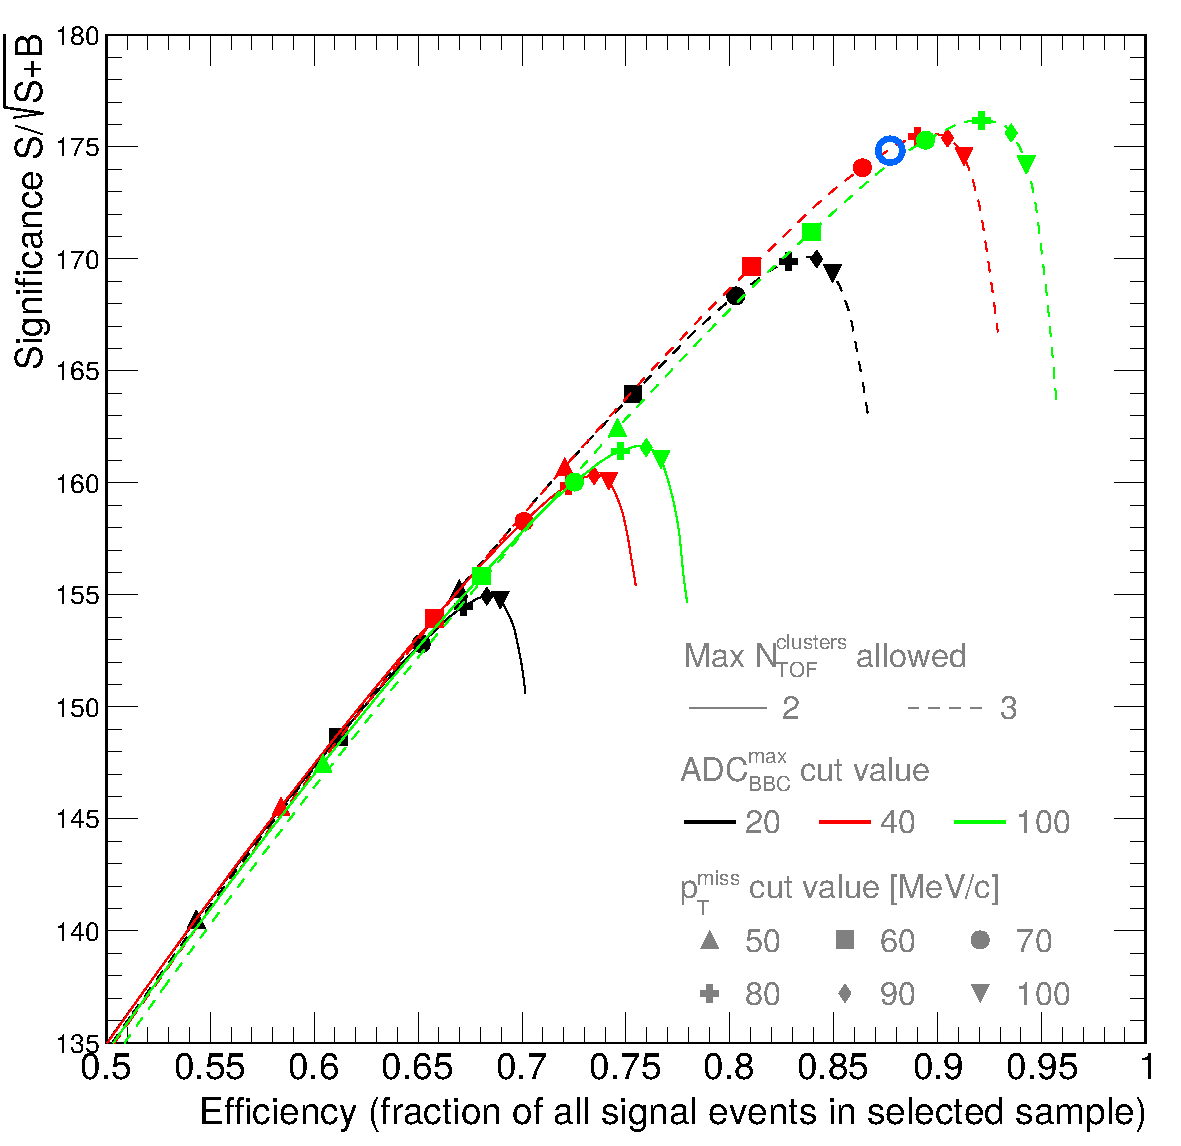
\includegraphics[width=\linewidth]{graphics/eventSelection/SignificanceVsEfficiency_pTmiss.pdf}}
  \end{subfigure}\\
  \begin{subfigure}[b]{\linewidth}\addtocounter{subfigure}{1}
                \subcaptionbox{\label{fig:EffVsBkgdFrac}}{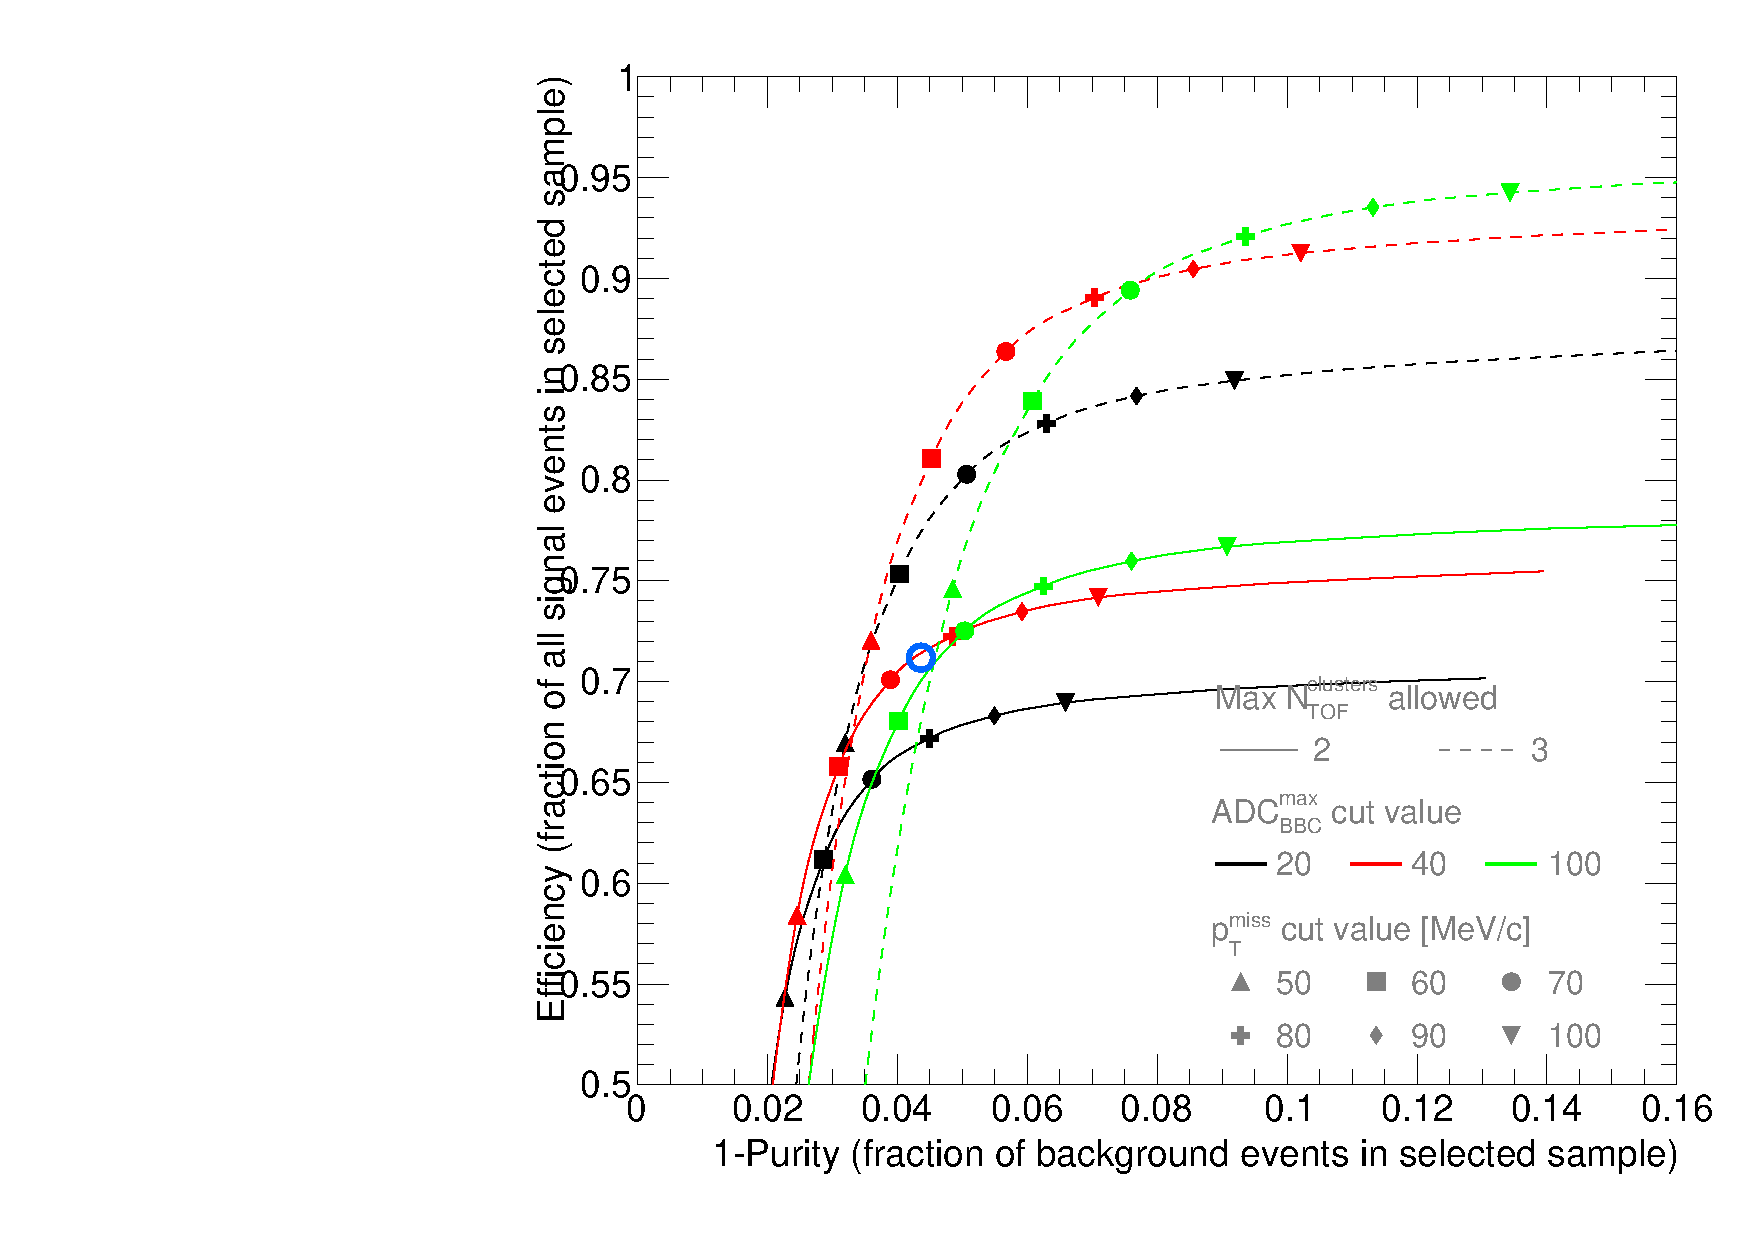
\includegraphics[width=\linewidth]{graphics/eventSelection/ROC_pTmiss.pdf}}
  \end{subfigure}
}%
\quad\quad%
\parbox{0.4725\textwidth}{
  \centering
  \begin{subfigure}[b]{\linewidth}\addtocounter{subfigure}{-2}
                \subcaptionbox{\label{fig:SignificanceVsBkgdFrac}}{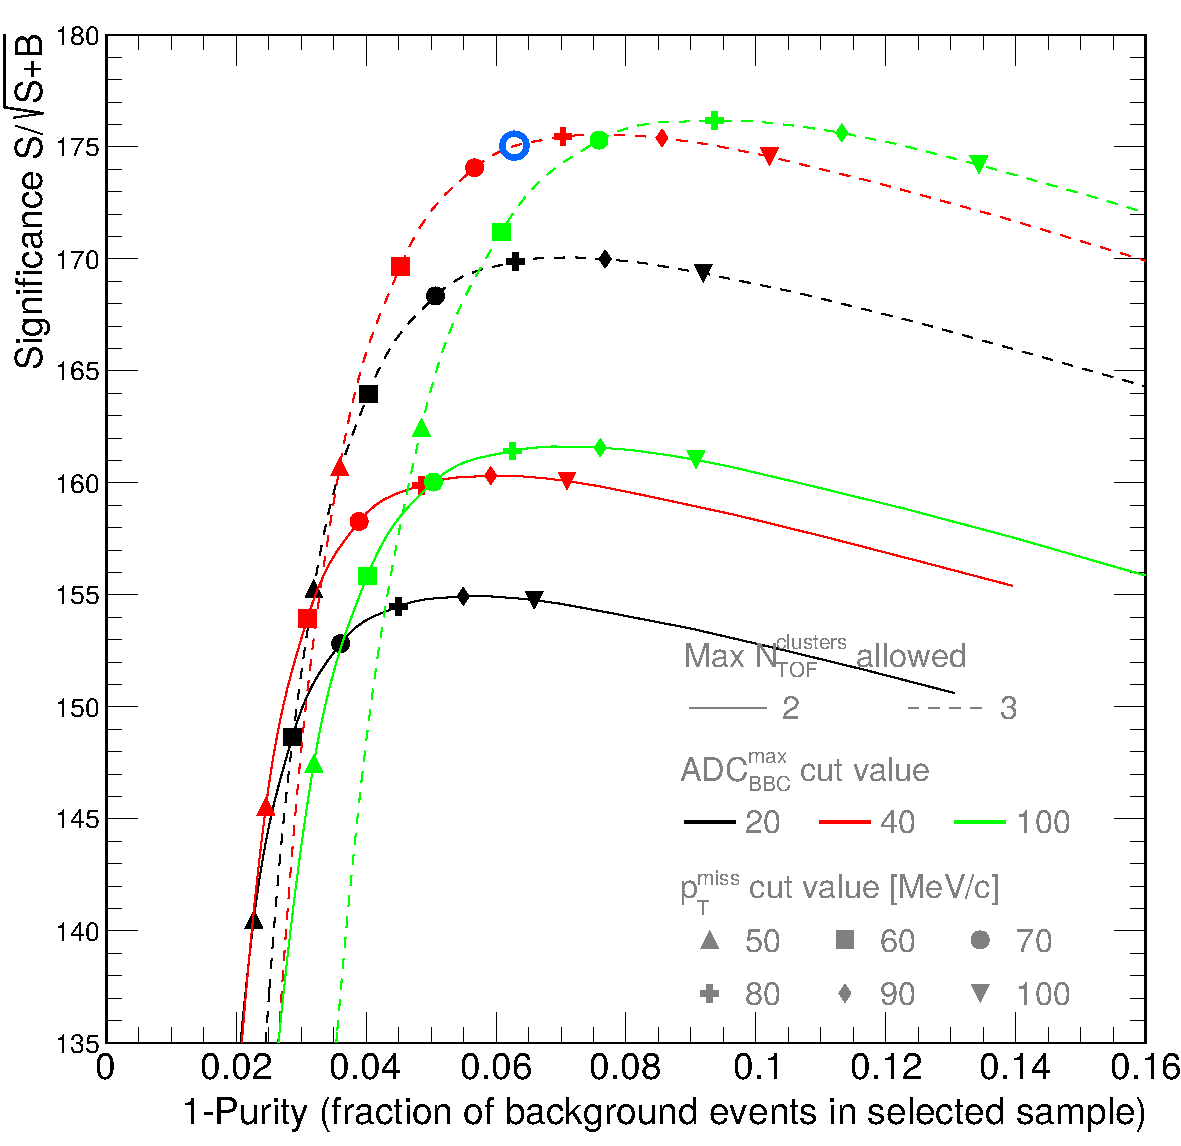
\includegraphics[width=\linewidth]{graphics/eventSelection/BkgdFractionVsEfficiency_pTmiss.pdf}}
  \end{subfigure}\\
  \begin{minipage}[t][1.042\linewidth][t]{\linewidth}\vspace{10pt}
    \caption[Relation between $\pi^{+}\pi^{-}$ significance, efficiency and purity vs. thresholds in cuts~\ref{enum:CutBbcLarge}, \ref{enum:CutTofClusters} and \ref{enum:CutMissingPt}]{Relation between $\pi^{+}\pi^{-}$ signal significance and efficiency (\subref{fig:SignificanceVsEff}), significance and purity (\subref{fig:SignificanceVsBkgdFrac}), and efficiency and purity (\subref{fig:EffVsBkgdFrac}) as a function of cut thresholds (the same for all channels) in BBC-large veto (\ref{enum:CutBbcLarge}), TOF cluster limit (\ref{enum:CutTofClusters}) and exclusivity cut (\ref{enum:CutMissingPt}). Lines show forementioned relations with changing $p_{T}^\text{miss}$ cut whose some specific values are indicated with different markers. Color denotes ADC threshold in BBC-large veto (black, red or green). Style of line (solid or dashed) denotes $N^{\text{TOF}}_{\text{clstrs}}$ limit. Working point considered optimal is marked with opened blue circle.}\label{fig:workingPoint}
  \end{minipage}
}%

\end{figure}\\
%--------------------------- 
In these equations $N_{\text{signal}}^{\text{cut}}$ is number of signal events in finally selected CEP $\pi^{+}\pi^{-}$ events, $N_{\text{bkgd}}^{\text{cut}}$ is number of non-exclusive background events in selected sample, and $N_{\text{signal}}^{\text{no~cut}}$ is number of signal events in sample after all cuts except the three studied cuts. These numbers were estimated using method described in Sec.~\ref{sec:nonExclBkgdDetermination}.

Relations between defined quantities are shown in Fig.~\ref{fig:workingPoint}. The first important observation was that allowing 3 TOF clusters instead of 2 (at fixed cuts~\ref{enum:CutBbcLarge} and~\ref{enum:CutMissingPt}) gives increase to selection efficiency by about 0.2, with only 0.01-0.02 decrease of the purity. We therefore decided to use condition $N^{\text{TOF}}_{\text{clstrs}}\leq 3$ in cut~\ref{enum:CutTofClusters}. 

In the next step the value of maximum $p_{T}^{\text{miss}}$ was found. From Fig~\ref{fig:workingPoint} one can read that with $N^{\text{TOF}}_{\text{clstrs}}\leq 3$ (dashed lines) the best balance between efficiency and purity is found for $p_{T}^{\text{miss}}$ cut value ranging between 60~MeV (rectangle) and 80~MeV (cross). We considered optimal threshold value of total transverse momentum $p_{T}^{\text{miss}}$ at 75~MeV which corresponds to 2.5$\sigma$, as elaborated in section devoted to exclusivity cut (\ref{enum:CutMissingPt}, Sec.~\ref{sec:C9}).

With fixed maximum number of TOF clusters and maximum $p_{T}^{\text{miss}}$ the maximum ADC in BBC-large was established. Similarly to previous paragraph, the best balance between efficiency and purity was found for ADC threshold of 40.

Certainly, not only factors considered here should be studied to find optimum working point, also e.g. size of systematic uncertainties for each cut value should be checked. Nonetheless, systematics related to these cuts are minor comparing to leading systematic uncertainties, therefore it was safe to ommit it.
